% !Mode\dots ``TeX:UTF-8''
% !TEX root = ../bare_jrnl.tex
\section{The online observability of \BCNs}
\label{sec:online}


In this section we propose the online observability to solve the problem mentioned in {\em Section \ref{sec:pre}}, and we will introduce its related information in detail. 

In the rest of this section, firstly we introduce the inspiration for the online observability. Secondly we define derivation function. Thirdly we present the definition of $k$-step determinability. Fourthly, we give the formal definition of the online observability of \BCNs\ by derivation function and $k$-step determinability. Finally, we compare the online observability with four existing observability.
%\begin{definition}
	 %In the online observability we determine the state of \BCN\ by observing its output sequence and then deriving and deciding the input sequence at every time step. What is more, this process can be accomplished in finite time steps.
%\end{definition}  without presupposing the initial state of \BCN


\subsection{Inspiration}


As we mentioned in {\em Section \ref{sec:pre}}, we can use the third existing observability to determine the initial state of \BCN. But in the third observability, a \BCN\ is observable unless there exists an finite input sequence $\mathsf{I}\in(\Delta_M)^k$ that determine its initial state $\mathsf{s}(0)$. 

However, as we can derive the set of possible initial states $\mathsf{S}(0)$ by initial output $\mathsf{o}(0)$ we observe at time step $0$ 
\[\mathsf{S}(0)=\{\mathsf{s}(0)|\mathsf{s}(0)\in \Delta_N\ ,\ h( \mathsf{s}(0))=\mathsf{o}(0)\}.\]
And for every $\mathsf{S}^{i}(0)$ (corresponding to the $\mathsf{o}^{i}(0)$) we derived, if we can find an input sequence $\mathsf{I}^{i}\in(\Delta_M)^k$ for some $k>0$, such that for any distinct states $\mathsf{s}^{x}(0)$, $\mathsf{s}^{y}(0) \in \mathsf{S}^{i}(0)$ implies $(HF)^k_{\mathsf{s}^{x}(0)}(\mathsf{I^i})\neq (HF)^k_{\mathsf{s}^{y}(0)}(\mathsf{I^i})$,
then we can determine the initial state too. 
What is more, in this case, the requirements for a \BCN\ to determine its initial state would be easier to meet. Because the corresponding input sequences $\mathsf{I}^{i}$ of different sets of possible initial states $\mathsf{S}^{i}(0)$ can be different. While in the third existing observability the $\mathsf{I}^{i}$ has to be identical.

Furthermore, we can derive the set of possible states $\mathsf{S}(1)$ by the outputs $\mathsf{o}(0)$ and $\mathsf{o}(1)$ we observe at time step $0$ and $1$ respectively and the input $\mathsf{i}(0)$ that
\[\mathsf{S}(1)=\{\mathsf{s}(1)|\mathsf{s}(0)\in \mathsf{S}(0),\ \mathsf{s}(1)=f({\mathsf{i}(0)},{\mathsf{s}(0)}),\ h(\mathsf{s}(1))=\mathsf{o}(1)\}.\]

And for every $\mathsf{S}^{i}(1)$ we derived, 
\begin{itemize}
  \item if we can find an input sequence $\mathsf{I}^{i}\in(\Delta_M)^k$ for some $k>0$, such that for any distinct states $\mathsf{s}^{x}(1)$, $\mathsf{s}^{y}(1) \in \mathsf{S}^{i}(1)$ implies $(HF)^k_{\mathsf{s}^{x}(1)}(\mathsf{I^i})\neq (HF)^k_{\mathsf{s}^{y}(1)}(\mathsf{I^i})$;
  \item  and for every $\mathsf{s}^{x}(1)$ $\in \mathsf{S}^{i}(1)$ there exists only one corresponding $\mathsf{s}^{x}(0)$ $\in \mathsf{S}^{i}(0)$ such that $\mathsf{s}^{x}(1)=f({\mathsf{i}(0)},{\mathsf{s}^{x}(0)})$,
\end{itemize} 
then we can determine the initial state too. And in this case, the requirements for the \BCN\ to determine the initial state would be further easier to meet. Because the corresponding input sequences $\mathsf{I}^{i}$ of different sets of possible states $\mathsf{S}^{i}(1)$ which derived by the same $\mathsf{S}(0)$ can be different. 

Therefore, we have that if we utilize sets of possible states we derived more, it would be easier for a \BCN\ to meet the requirements to determine its initial state. According to this rule, we propose the online observability. Instead of finding the input sequence $\mathsf{I}$ before we take the procedure of determining the initial state. In the online observability we use the $\mathsf{S}(t)$ (which will be formally defined in the next subsection) we derive at every time step to adaptively contruct the input sequence to determine the initial state of \BCNs. Such that the requirements to determine the \BCNs' initial state would be easiest to meet. Thus, a \BCN\ satisfies the online observability iff its initial state $\mathsf{s}(0)$ can be determined for every $\mathsf{s}(0) \in \Delta_N$.

%\tl{do not understand this at all, what does it mean by harsh?}

%The reason why we called this type of observability online observability because in the process of determining the initial state of \BCNs, we use the outputs we observe to construct the input sequence at every time step. Thus the construction of the input sequence is adaptive. By this way, we can make full use of the outputs and inputs to determine the initial state of \BCNs. %We call this property {\em interactivity}. With the {\em interactivity}, we called this type of observability online observability.
%\begin{itemize}
 % \item Firstly, in the online observability, we determine the initial state of \BCNs\ in real time. In other words, we only need one test case to determine the initial state of \BCNs. We call this property {\em real-time} property.%Such that we can determine the initial state of any test case of \BCNs.
%  \item  Secondly, in the online observability, we use the outputs we observe to derive and decide the input sequence at every time step in the process of determining the initial state of \BCNs. By this way, we can make full use of the outputs and inputs to determine the initial state of \BCNs. We call this property {\em interactivity}.
%\end{itemize} 

%\tl{basically this is to say that the selection of the input string is adaptive?}

%We need the {\em real-time} property to help us avoid repeating biological experiments, and the {\em real-time} property makes the online observability be the sufficient condition of determine the initial state $s_o$ of \BCNs\ in real time. However, the {\em interactivity} would help us to find the necessary condition by making full use of the outputs and inputs to determine the initial state of \BCNs. 

%\tl{maybe I did not understand this, but I think you are confusing two things: the observability and the algorithm (approach) to determine the initial state. It seems to me that you are describing a new approach (the online approach), but does this change the observability? if yes, how? Is this a stronger notion or a weaker notion or incomparable?}

%The observability we propose can determine the initial state online.
 %Because in the process of determining the initial state every input of the input sequence is decided by the output we observe at every time step. 
After introducing the idea of the online observability, we briefly present how to determine the initial state of a \BCN. At every time setp $t$, 
\begin{itemize}
\item firstly, we observe the output $\mathsf{o}(t)$ of \BCN, then based on the relation $\mathsf{o}(t)=h(\mathsf{s}(t))$ we can infer the set of possible states $\mathsf{S}(t)$ by the $\mathsf{o}(t)$.
\item Secondly, with the set of possible states $\mathsf{S}(t)$ we can derive the set of possible inputs $\{\mathsf{i}_x(t),\ldots,\mathsf{i}_y(t)\}$, such that for every $\mathsf{i}^{i}(t)\in \{\mathsf{i}_x(t),\ldots,\mathsf{i}_y(t)\}$ we have  for any distinct $\mathsf{s}^{z}(t)$, $\mathsf{s}^{w}(t) \in \mathsf{S}(t)$, they will not become the same state after being affected by this input $\mathsf{i}^{i}(t)$ i.e., $f(\mathsf{s}^{z}(t), \mathsf{i}^{i}(t))\neq f(\mathsf{s}^{w}(t),\mathsf{i}^{i}(t))$.  And then, we choose an input $\mathsf{i}(t)$ from $\mathsf{I}(t)$.
\item Thirdly, based on the relation $\mathsf{s}(t+1)= f({\mathsf{i}(t)},{\mathsf{s}(t)})$, the set of possible states $\mathsf{S}(t+1)$ of next time step ($t+1$) is preliminarily derived by the input $\mathsf{i}(t)$ we chose. 
\end{itemize} 
 %Then as we can know the possible states set
 The cardinal number of possible states set does not change or decrease in the determining process i.e., $|\mathsf{S}(t+1)|\le|\mathsf{S}(t)|$. % (will be shown in {\em Example \ref{exa:8}}). 
 If the cardinal number of possible states set $|\mathsf{S}(t)|=1$, then we can determine the $\mathsf{s}(t)$. And then because for every $\mathsf{s}^{i}(t)\in $ $\mathsf{S}(t)$ there is exact one corresponding $\mathsf{s}^{i}(t-1)\in $ $\mathsf{S}(t-1)$ we can determine $\mathsf{s}(t-1)$, $\mathsf{s}(t-2)$, \ldots, and $\mathsf{s}(0)$.

Therefore, in the definition of online observability, 
\begin{itemize}
\item firstly we need to describe how to derive the set $\mathsf{S}(t)$ of possible states of the \BCN\ by the output and input at every time step $t$. So we define the derivation function to solve this problem.
\item  Secondly, we need to describe with a set of possible initial states $\mathsf{S}(0)$ whether or not we can determine the initial state $\mathsf{s}(0)$ for every $\mathsf{s}(0) \in \mathsf{S}(0)$ by the above mentioned process in $k$ time steps, thus we define the $k$-step determinability for $\mathsf{S}(t)$. 
\end{itemize} 

Therefore, we have the definition of the online observability that a \BCN\ is online observable if for every $\mathsf{S}^{i}(0)$ we derived, there exists a $k^i\ge 0$ such that the $\mathsf{S}^{i}(0)$ is $k^i$-step determinable.

% In the rest of this section, firstly we define derivation function. Secondly we present the definition of $k$-step determinability (before $K$-step determinability). Thirdly, we give the formal definition of the online observability of \BCNs\ by derivation function and $K$-step determinability. Finally, we compare the online observability with four existing observability.
\subsection{Derivation function}
%Different from four existing observabilities, t

 
 % After deciding input, we can observe the new output, and then we can infer the new possible states set.
In order to better describe how to derive the set of possible states $\mathsf{S}(t)$ and the set of possible inputs $\mathsf{I}(t)$ at every time step $t$, we propose the derivation function. The definition of it is as follows.
%$\Ded\left(S, i, o\right)$
\begin{definition}[Derivation Function] 
In a Boolean control network, let
\begin{itemize}
\item $2^{\Delta_N}$ be the power set of states; 
\item $(\Delta_M\cup\varepsilon)$ be the set of inputs and $\varepsilon$ means empty input; 
\item $(\Delta_Q\cup\varepsilon)$ be the set outputs and $\varepsilon$ means empty output.
\end{itemize} 
A derivation function \[\Ded:2^{\Delta_N}\times (\Delta_M\cup\varepsilon) \times (\Delta_Q\cup\varepsilon) \mapsto 2^{\Delta_N}\] %Based on derivation process mentioned before, 
with the following properties. 
	%\tl{it is quite unusual that a def depends on the process...}
	%for every $S\in 2^{\Delta_N}$ 
	That for each element $\mathsf{s}'\in \Ded\left(\mathsf{S}, \mathsf{i}, {o}\right)$ there exists a corresponding $\mathsf{s}\in \mathsf{S}$ of $\mathsf{s}'$ such that 
	%\tl{but here you are defining something?!}
%\[s=L\ltimes i\ltimes s'\ when\ i\neq \varepsilon, \] 

\[\mathsf{s}'=\left\{
\begin{array}{rcl}
f( \mathsf{i}, \mathsf{s})      &      & {\mathsf{i}\neq \varepsilon}\\
\mathsf{s}       &      & {\mathsf{i}= \varepsilon}
\end{array} \right. \]

and 

\[h(\mathsf{s}')=\mathsf{o}\ when\ \mathsf{o}\neq \varepsilon.\]

\end{definition}
%where   
%\begin{itemize}
 % \item $S\in 2^{\Delta_N}$ is a set of possible states ;
%  \item $i\in (\Delta_M\cup\varepsilon)$ represents the input;
 % \item $o\in(\Delta_Q\cup\varepsilon)$ represents the output; 
  %\item $\Ded\left(S, i, o\right)\in 2^{\Delta_N}$ is the set of possible states determined by derivation function.
%\end{itemize} 

%\tl{for me this def is well-defined, so I could not really understand the rest}
 
% We utilize the derivation functon $\Ded\left( \mathsf{S},  \mathsf{i},  \mathsf{o}\right)$ to represent various kinds of information derived by $ \mathsf{S}$, $ \mathsf{i}$ and $ \mathsf{o}$. 
\begin{example}
 In order to better illustrate the derivation functon $\Ded\left( \mathsf{S},  \mathsf{i},  \mathsf{o}\right)$, we use the \BCN\ mentioned in {\em Example \ref{exa:2}} as an example to apply this function. %We can know the details of the derivation function better by researching this example.
 
 For all $\mathsf{i}^{i}\in \Delta_M$ and for all $\mathsf{o}^{j}\in \Delta_Q$ we have 
\begin{equation*}
\begin{split}
\Ded\left(\emptyset,\mathsf{i}^{i},\mathsf{o}^{j}\right)=\emptyset\\
%D\left(\varnothing,I_i,O_i\right)=D\left(\varnothing,\varepsilon,O_i\right)= &D\left(\varnothing,\varepsilon,\varepsilon\right)=\varnothing\\
\end{split}
\label{equ:7}
\end{equation*}

This equation represents that 
%if the possible states set is an empty set of states $\emptyset$, then no matter what we input and observe we can only deduce the possible set is the empty set $\emptyset$. It means that 
if we don't know any information about the state of a \BCN, then we can not deduce anything no matter what we input and observe.

For all $\mathsf{S}^{i}\in 2^{\Delta_N}$ we have 
\begin{equation*}
\begin{split}
\Ded\left(\mathsf{S}^{i},\varepsilon,\varepsilon\right)=\mathsf{S}^{i}\\
\end{split}
\label{equ:8}
\end{equation*}

 This equation represents that %, we have that for any possible states set $\mathsf{S}^{i}$, and we neither input anything nor observe the output of \BCN. In this case we can only deduce that the possible states set is $\mathsf{S}^{i}$. It means that 
 we can not know more information about a \BCN\ than what we knew before before we observe the output and decide the input.
\begin{equation*}
\begin{split}
\Ded\left(\Delta_N,\varepsilon,\delta_4^0\right)=&\{\delta_{16}^0,\delta_{16}^1,\delta_{16}^2\}\\
\end{split}
\label{equ:9}
\end{equation*}
%\tl{is this an example?}
 
In this equation, the possible states set $\mathsf{S}=\Delta_N$, and  we observe that the outputs of \BCN\ is $\delta_4^0$ before we decide the input. In this case we can derive that the state can be $\delta_{16}^0$, $\delta_{16}^1$ or  $\delta_{16}^2$. This equation shows how to derive the set of possible states by observing the output at every time step. So we have that the cardinal number of the possible states set may decrease after we observe the output of \BCN. As the cardinal number of the set possible states decreasing, we can further determine the range of values for the initial state. 
\begin{equation*}
\begin{split}
\Ded\left(\{\delta_{16}^0,\delta_{16}^1,\delta_{16}^2\},\delta_4^0,\varepsilon\right)=&\{\delta_{16}^{9},\delta_{16}^3,\delta_{16}^{10}\}\\
\end{split}
\label{equ:10}
\end{equation*}

And then, if the possible states set $\mathsf{S}=\{\delta_{16}^0$, $\delta_{16}^1$, $\delta_{16}^2\}$ and we input $\delta_4^0$. Before we observe the output of the \BCN\ we can only derive that the possible states would be $\delta_{16}^{9}$, $\delta_{16}^3$ or  $\delta_{16}^{10}$. In this equation, the cardinal number of the possible states set does not decrease before we observe the output of this \BCN. Thus, for every $\mathsf{s}'\in\{\delta_{16}^{9},\delta_{16}^3,\delta_{16}^{10}\}$ there exists only one corresponding $\mathsf{s}\in\{\delta_{16}^{0},\delta_{16}^1,\delta_{16}^{2}\}$ such that $\mathsf{s}'=f( \delta_4^0, \mathsf{s})$.%That for every $\mathsf{s}'\in \Ded\left(\mathsf{S}, \mathsf{i}, \varepsilon \right)$, there exists only one corresponding $\mathsf{s}\in \mathsf{S}$ of $\mathsf{s}'$ such that $\mathsf{s}'=L\ltimes \mathsf{i}\ltimes \mathsf{s}$. 
%Therefore the input $\delta_4^1$ is a suitable input, this equation shows how to derive the set of possible inputs. And it would help us derive the set possible inputs $\mathsf{I}(t)$. Therefore, the derivation function would make the online obervability satisfy the {\em interactivity}.
\begin{equation*}
\begin{split}
\Ded\left(\{\delta_{16}^0,\delta_{16}^1,\delta_{16}^2\},\delta_4^0,\delta_4^2\right)=&\{\delta_{16}^{9},\delta_{16}^{10}\}\\
\end{split}
\label{equ:11}
\end{equation*}

And then if we observe that the output of \BCN\ is $\delta_4^2$, we can deduce that the possible state can be $\delta_{16}^{9}$ or  $\delta_{16}^{10}$ shown in this equation. 
\begin{equation*}
\begin{split}
\Ded\left(\{\delta_{16}^3,\delta_{16}^4,\delta_{16}^5,\delta_{16}^6\},\delta_4^3,\varepsilon\right)=&\{\delta_{16}^8,\delta_{16}^{7},\delta_{16}^{10}\}
\end{split}
\label{equ:12}
\end{equation*}

 Finally if the set of possible states $\mathsf{S}=\{\delta_{16}^3, \delta_{16}^4, \delta_{16}^5, \delta_{16}^6\}$ and the inputs is $\delta_4^3$. Before we observe the output of \BCN\ we can derive that the possible states should be $\delta_{16}^8$, $\delta_{16}^7$ or $\delta_{16}^{10}$ shown in this equation. Because both $\delta_{16}^3$ and $\delta_{16}^4$ become $\delta_{16}^8$ after affected by $\delta_4^3$, we can not distinguish them anymore.   %In this equation, the cardinal number of the possible states set decrease before we observe the output of this \BCN.% And if the current state of the \BCN\ is one of them then we can not determine the  state any more. Therefore, the derivation function helps us define the online obervability to satisfy the {\em real-time} property. 
 \label{exa:8}
 \end{example}   
 
 Then for a \BCN, we have the set of possible states of it $\mathsf{S}(t)$ is defined as follows.
 \begin{definition}[$\mathsf{S}(t)$] In a \BCN, with the input sequence $\mathsf{i}(0)\mathsf{i}(1)\ldots\mathsf{i}(k-1)$ and output sequence $\mathsf{o}(0)\mathsf{o}(1)\ldots\mathsf{o}(k)$, for every $0\le t\le k$, we have
	\[\mathsf{S}(t)=\left\{
\begin{array}{rcl}
\Ded\left(\Delta_N,\varepsilon,\mathsf{o}(0)\right)      &      & {t=0}\\
\Ded\left(\mathsf{S}(t-1),\mathsf{i}(t-1),\mathsf{o}(t)\right)       &      & {t>0}
\end{array} \right. \]

\end{definition}
 
 As the derivation function can only describe the process of deriving the set possible states $\mathsf{S}(t)$ of \BCNs\ at every time step. But we need to know how to choose the input at every time step to determine the initial state of \BCNs. Thus we propose the $k$-step determinability for the set of possible states $\mathsf{S}(t)$ to depict whether we can determine the state $\mathsf{s}(t)$ in $k$ time steps for every $\mathsf{s}(t)\in \mathsf{S}(t)$.
\subsection{$k$-step determinability}
After we difined the derivation function, we present the definition of $k$-step determinability for the set of possible states $\mathsf{S}(t)$, where the $k\ge 0$. % It may easier to difine online observability by programming language. But we would like to define its mathematical form for preciseness of concepts. However, before defining the online observability of \BCNs, we need to difine the $k$-step determinability of the states set of \BCNs\ at first.
\begin{definition}[$k$-Step Determinability] 

When $k=0$, a set of possible states $\mathsf{S}(t)$ is $0$-step determinable if $|\mathsf{S}(t)|=1$. 

When $k>0$, a set of states $\mathsf{S}(t)$ is $k$-step determinable
 if $|\mathsf{S}(t)|>0$ and for $\mathsf{S}(t)$ there exists an input $\mathsf{i}^{i}(t) \in \Delta_M$ such that
 \begin{itemize}
 \item  $|\Ded\left(\mathsf{S}(t),\mathsf{i}^{i}(t),\varepsilon\right)|=|\mathsf{S}(t)|$, and 
 \item  for each \[\mathsf{o}^{j}(t+1)\in \Delta_Q\] such that \[|\Ded\left(\mathsf{S}(t),\mathsf{i}^{i}(t),\mathsf{o}^{j}(t+1)\right)|\neq 0,\] there exists a ${k'}<k$ such that $\Ded\left(\mathsf{S}(t),\mathsf{i}^{i}(t),\mathsf{o}^{j}(t+1)\right)$ is $k'$-step determinable.
 \end{itemize}
 %And we default $k\ge0$ when we talk about whether a states set of \BCNs\ $S$ is $k$-step deterministic or not.
\end{definition}

% In the time step $t$ and $S$ is the set of current possible states we derived.
%The $k$-step determinability depict whether we can determine $\mathsf{s}(t)$ by the the set of possible states $\mathsf{S}(t)$ in $k$ time steps for every $\mathsf{s}(t) \in \mathsf{S}(t)$. 
After defining the $k$-step determinability, we illustrate why it defined by this way.
\begin{itemize}
\item When $k=0$, and we can determine the state $\mathsf{s}(t)$ at time step $t+k$ for every $\mathsf{s}(t)\in \mathsf{S}(t)$. To guarantee this, we have $|\mathsf{S}(t)|=1$. Only in this case we can determine the state $\mathsf{s}(t)$ at time step $t$. 

Therefore, the $k$-step determinability is well defined when $k=0$.

\item  If for $k=0,\ldots, p$ the $k$-step determinability is well defined, where $p\ge 0$. When $k=p+1$, and we can determine the state $\mathsf{s}^{i}(t)$ at time step $t+(p+1)$ for every $\mathsf{s}^{i}(t)\in \mathsf{S}(t)$. To guarantee this, we have for $\mathsf{S}(t)$ there exists an input $\mathsf{i}^{i}(t) \in \Delta_M$ such that
\begin{itemize}
\item $|\Ded\left(\mathsf{S}(t),\mathsf{i}^{i}(t),\varepsilon\right)|=|\mathsf{S}(t)|$, only in this case we can determine the state $\mathsf{s}^{i}(t)$ at time step $t+(p+1)$ for every $\mathsf{s}^{i}(t)\in \mathsf{S}(t)$ when we can determine its corresponding state $\mathsf{s}^{i}(t+1)$ at time step $(t+1)+p$.
\item And we can determine the state $\mathsf{s^{i}}(t+1)$ at time step $(t+1)+p$ for every \[\mathsf{s}^{i}(t+1)\in \Ded\left(\mathsf{S}(t),\mathsf{i}^{i}(t),\varepsilon\right).\] To guarantee this we have for each \[\mathsf{o}^{j}(t+1)\in \Delta_Q\] such that \[|\mathsf{S}^{j}(t+1)|=|\Ded\left(\mathsf{S}(t),\mathsf{i}^{i}(t),\mathsf{o}^{j}(t+1)\right)|\neq 0,\] there exists a ${k'}\le p=k-1$ such that \[\mathsf{S}^{j}(t+1)=\Ded\left(\mathsf{S}(t),\mathsf{i}^{i}(t),\mathsf{o}^{j}(t+1)\right)\] is $k'$-step determinable. Only in this case we can determine every state $\mathsf{s}^{i}(t+1)$ at time step $(t+1)+p$.
 \end{itemize}
Therefore, the $k$-step determinability is well defined when $k=p+1$. And the input $\mathsf{i}^{i}(t)$ is an input which makes $\mathsf{S}(t)$ $k$-step determinable, we can chose it to determine $\mathsf{s}(t)$.

 \end{itemize}
 
For $\mathsf{S}(t)$, the $k$-step determinability is well defined when $k=0$. And if for $k=0,\ldots p$ the $k$-step determinability is well defined, the $k$-step determinability is also well defined when $k=p+1$. Therefore, we have the $k$-step determinability is well defined for every $k\ge 0$.
 
 Then, in order to better illustrate this definition, we give the following example.
\begin{example}
In the \BCN\ mentioned in {\em Example \ref{exa:2}}. For the set of possilble states $\Ded\left(\Delta_N,\varepsilon,\delta_4^0\right)=\{\delta_{16}^0,\delta_{16}^1,\delta_{16}^2\}$, the cardinality number of this set $|\{\delta_{16}^0,\delta_{16}^1,\delta_{16}^2\}|=3>1$, and for this set there exists $\delta_{4}^3$ such that 
 \begin{itemize}
 \item  $|\Ded\left(\{\delta_{16}^0,\delta_{16}^1,\delta_{16}^2\},\delta_{4}^3,\varepsilon\right)|=|\{\delta_{16}^0,\delta_{16}^{13},\delta_{16}^6\}|$,
 \item   and for each $\mathsf{o}^{j}\in \Delta_Q$
  \begin{itemize}
  \item   $|\Ded\left(\{\delta_{16}^0,\delta_{16}^1,\delta_{16}^2\},\delta_{4}^3,\delta_{4}^0\right)|=|\{\delta_{16}^0\}|=1$, that the $\{\delta_{16}^0\}$ is $0$-step deterministic;
 \item  $|\Ded\left(\{\delta_{16}^0,\delta_{16}^1,\delta_{16}^2\},\delta_{4}^3,\delta_{4}^3\right)|=|\{\delta_{16}^{13}\}|=1$, that the $\{\delta_{16}^{13}\}$ is $0$-step deterministic;
  \item  $|\Ded\left(\{\delta_{16}^0,\delta_{16}^1,\delta_{16}^2\},\delta_{4}^3,\delta_{4}^1\right)|=|\{\delta_{16}^{6}\}|=1$, that the $\{\delta_{16}^{6}\}$ is $0$-step deterministic.
 \end{itemize}
 \end{itemize}
 Therefore the set of states $\{\delta_{16}^0,\delta_{16}^1,\delta_{16}^2\}$ is $1$-step deterministic.
\label{exa:9}
\end{example}  

In addition, we propose some lemmas for the $k$-step determinability.
\begin{comment}
\begin{lemma}
 In the time step $t$ and $S$ is the set of current possible states we derived. If $S$ is $k$-step deterministic, then we can determine the current state $s(t)$ of this \BCN\ for every $s(t)\in S$ in real time at time step ($t+k$).
  \label{lemm:6}
\end{lemma}

\begin{proof} If $k=0$, then we have $|S|=1$. Therefore, we can determine the current state $s(t)$ of this \BCN\ in real time at time step $t$, and then the {\em Lemma \ref{lemm:6}} is right. 

If for $k=0,\ldots k=p$ the {\em Lemma \ref{lemm:6}} is right. When $k=p+1$ and the $S$ is $k$-step deterministic, then we have for this set of states $S$ there exists $i_p \in \Delta_M$ such that
 \begin{itemize}
 \item  $|\Ded\left(S,i_p,\varepsilon\right)|=|S|$, and 
 \item  for each $o_j$ in $\Delta_Q$ such that $|\Ded\left(S,i_p,o_j\right)|\neq 0$ there exists a ${k'}<(p+1)$ that $\Ded\left(S,i_p,o_j\right)$ is $k'$-step deterministic.
 \end{itemize}
 However, for $k=0,\ldots k=p$ the {\em Lemma \ref{lemm:6}} is right, thus we can determine the state $s(t+1)$ of this \BCN\ for every $s(t+1)\in \Ded\left(S,i_p,\varepsilon\right)$ in real time at time step $(t+1+k')$. What is more, we have $|\Ded\left(S,i_p,\varepsilon\right)|=|S|$, then for every $s(t+1)\in \Ded\left(S,i_p,\varepsilon\right)$ we can find the corresponding one $s(t)$ for it. So we can determine the state $s(t)$ of this \BCN\ for every $s(t)\in S$ in time step $(t+p+1)$. So we have if for $k=0,\ldots k=p$ the {\em Lemma \ref{lemm:6}} is right then the {\em Lemma \ref{lemm:6}} is right too when $k=p+1$. 
 
The {\em Lemma \ref{lemm:6}} is right when $k=0$, and if for $k=0,\ldots k=p$ the {\em Lemma \ref{lemm:6}} is right then the {\em Lemma \ref{lemm:6}} is right too when $k=p+1$. Thus we have the {\em Lemma \ref{lemm:6}} is right for any $k\in \mathbb{N}$.
\end{proof}

The {\em Lemma \ref{lemm:6}} indicates that for the set of current possible states $S$ we derived, $S$ is $k$-step deterministic is the sufficient condition of determine the current state $s(t)$ of this \BCN\ for every $s(t)\in S$ in real time at time step ($t+k$). Therefore, the $k$-step determinability helps us define the online obervability to satisfy the {\em real-time} property. 
\begin{lemma}
 In the time step $t$ and $S$ is the set of current possible states we derived. If we can determine the current state $s(t)$ of this \BCN\ for every $s(t)\in S$ in real time in time step $t+k$, then $S$ is $k$-step deterministic. 
  \label{lemm:7}
\end{lemma}

\begin{proof}
If $k=0$ and we can determine the current state $s(t)$ of this \BCN\ for every $s(t)\in S$ in time step $t$. So we have $|S|=1$, and then $S$ is $0$-step deterministic. Therefore, we have the {\em Lemma \ref{lemm:7}} is right when $k=0$. 

If for $k=0,\ldots k=p$ the {\em Lemma \ref{lemm:7}} is right. When $k=p+1$ and we can determine the current state $s(t)$ of this \BCN\ for every $s(t)\in S$ in real time in time step $t+k$, then from the {\em Lemma \ref{lemm:1}} we have for this set of states $S$ there exists $i_p \in \Delta_M$ such that $|\Ded\left(S,i_p,\varepsilon\right)|=|S|$. And $s(t+1)$ can be determined in time step $(t+1+p)$ for every $s(t+1)\in \Ded\left(S,i_p,\varepsilon\right)$. Then we have that for each $o_j$ in $\Delta_Q$ such that $|\Ded\left(S,i_p,o_j\right)|\neq 0$ there exists a ${k'}<(p+1)$ that $\Ded\left(S,i_p,o_j\right)$ is $k'$-step deterministic.
Therefore, we have $S$ is $(p+1)$-step deterministic. And then have if for $k=0,\ldots k=p$ the {\em Lemma \ref{lemm:7}} is right then the {\em Lemma \ref{lemm:7}} is right too when $k=p+1$. 

The {\em Lemma \ref{lemm:7}} is right when $k=0$, and if for $k=0,\ldots k=p$ the {\em Lemma \ref{lemm:7}} is right then the {\em Lemma \ref{lemm:7}} is right too when $k=p+1$. Thus we have the {\em Lemma \ref{lemm:7}} is right for any $k\in \mathbb{N}$.
\end{proof}

The {\em Lemma \ref{lemm:7}} indicates that for the set of current possible states $S$ we derived, $S$ is $k$-step deterministic is the necessary condition of determine the current state $s(t)$ of this \BCN\ for every $s(t)\in S$ in real time at time step ($t+k$). Therefore, the $k$-step determinability helps us define the online obervability to satisfy the {\em interactivity}. 
%Therefore if we can determine the infimum of $k$ for a set of states $S$, we would find the length of the shortest path to determine the state of a \BCN\ by this possible states set $S$.


\begin{lemma}
 If a set of possible states $\mathsf{S}^{x}(t)$ is $k^1$-step determinable and $k^1< k^2$, then $\mathsf{S}^{x}(t)$ is $k^2$-step determinable. %But if the states set $S$ is $k_1$-step deterministic and $k_1> k_2$, we can not deduce that $S$ is $k_2$-step deterministic. 
  \label{lemm:2}
\end{lemma}

\begin{proof}
 A set of possible states $\mathsf{S}^{x}(t)$ is $k^1$-step determinable and the $k^1< k^2$. 
 
 If $k^1=0$ then $|\mathsf{S}^{x}(t)|=1$. Therefore for $\mathsf{S}^{x}(t)$ there exists $i_p$ in $\Delta_M$ such that
 \begin{itemize}
 \item  $|\Ded\left(\mathsf{S}^{x}(t),\mathsf{i}^{i}(t),\varepsilon\right)|=|\mathsf{S}^{x}(t)|=1$, and 
 \item  for each \[\mathsf{o}^{j}(t+1)\in \Delta_Q\] such that \[|\Ded\left(\mathsf{S}^{x}(t),\mathsf{i}^{i}(t),\mathsf{o}^{j}(t+1)\right)|=1\neq 0\] that $\Ded\left(\mathsf{S}^{x}(t),\mathsf{i}^{i}(t),\mathsf{o}^{j}(t+1)\right)$ is $k'$-step determinable where ${k'}=0=k^1< k^2$.
 \end{itemize}
 Therefore the set of states $\mathsf{S}^{x}(t)$ is $k^2$-step determinable.
 
 If $k_1>0$, then $|\mathsf{S}^{x}(t)|>0$, and for this set of states $\mathsf{S}^{x}(t)$ there exists $\mathsf{i}^{i}(t) \in \Delta_M$ such that
 \begin{itemize}
 \item  $|\Ded\left(\mathsf{S}^{x}(t),\mathsf{i}^{i}(t),\varepsilon\right)|=|\mathsf{S}^{x}(t)|$, and 
 \item  for each \[\mathsf{o}^{j}(t+1)\in \Delta_Q\] such that \[|\Ded\left(\mathsf{S}^{x}(t),\mathsf{i}^{i}(t),\mathsf{o}^{j}(t+1)\right)|\neq 0\] and $\Ded\left(\mathsf{S}^{x}(t),\mathsf{i}^{i}(t),\mathsf{o}^{j}(t+1)\right)$ is $k'$-step determinable where ${k'}<k^1< k^2$.
 \end{itemize}
 Therefore the set of states $\mathsf{S}^{x}(t)$ is $k^2$-step determinable.

 So we have the {\em Lemma \ref{lemm:2}} is right.
\end{proof}

However its inverse proposition is not true. Because, if the states set $\mathsf{S}^{x}(t)$ is $k^1$-step determinable and $k^1> k^2$. And for $\mathsf{S}^{x}(t)$ there is no such $\mathsf{i}^{i}(t) \in\Delta_M$ such that
 \begin{itemize}
 \item  $|\Ded\left(\mathsf{S}^{x}(t),\mathsf{i}^{i}(t),\varepsilon\right)|=|\mathsf{S}^{x}(t)|$, and 
 \item  for each \[\mathsf{o}^{j}(t+1)\in \Delta_Q\] such that \[|\Ded\left(\mathsf{S}^{x}(t),\mathsf{i}^{i}(t),\mathsf{o}^{j}(t+1)\right)|\neq 0\] and $\Ded\left(\mathsf{S}^{x}(t),\mathsf{i}^{i}(t),\mathsf{o}^{j}(t+1)\right)$ is $k'$-step determinable where ${k'}<k_2<k_1$.
 \end{itemize}
 Then the set of states $\mathsf{S}^{x}(t)$ is not $k_2$-step determinable.

From the {\em Lemma \ref{lemm:2}}, we know that there exists the minimum value of $k$ for the $k$-step determinability of a set of possible states $\mathsf{S}(t)$. It indicates the least time steps we need to definitely determine $\mathsf{s}(t)$ of a \BCN\ by $\mathsf{S}(t)$.
\begin{definition}[$k_{min}(\mathsf{S}(t))$] 
For a set of states $\mathsf{S}(t)$, if there exists a $k^i\ge0$ such that $\mathsf{S}(t)$ is $k^i$-step determinable but $\mathsf{S}(t)$ is not $(k^{i}-1)$-step determinable, then $k^{i}$ is the $k_{min}(\mathsf{S}(t))$ of $\mathsf{S}(t)$.
\end{definition}

In {\em Section \ref{sec:app}}, we will represent the details about finding the shortest path when we use the online observability to determine the initial state of a \BCN. %And some other some other advantages of the online observability.

%{\em Theorem \ref{theo:4}}

%We can consider ``A set of possible states $S$ is $K$-step deterministic'' as ``We can determine the state of a \BCN\ by this possible states set $S$ in finite steps''. Therefore we have some other theorems for the $K$-step determinability.

%We prove the {\em Lemma \ref{lemm:4}} at first.
\end{comment}
\begin{lemma}
For the sets of states $\mathsf{S}^{1}(t)$ and $\mathsf{S}^{2}(t)$, if $\mathsf{S}^{2}(t)$ is $k$-step determinable and $\mathsf{S}^{1}(t)\subseteq \mathsf{S}^{2}(t)$, then $\mathsf{S}^{1}(t)$ is $k$-step determinable.
  \label{lemm:4}
\end{lemma}
\begin{proof}
The set of states $\mathsf{S}^{2}(t)$ is $k$-step determinable and $\mathsf{S}^{1}(t)\subseteq \mathsf{S}^{2}(t)$. %Therefore we have $k>0$ from this precondition.

If $k=0$, we have \[|\mathsf{S}^{1}(t)|=|\mathsf{S}^{2}(t)|=1,\] and \[\mathsf{S}^{1}(t) = \mathsf{S}^{2}(t).\] Therefore, we have $\mathsf{S}^{1}(t)$ is $0$-step determinable, thus we have the {\em Lemma \ref{lemm:4}} is right when $k=0$.


 
 If for $k=0,\ldots, p$ the {\em Lemma \ref{lemm:4}} is right. When $k=p+1$, we have for $\mathsf{S}^{2}(t)$ there exists a $\mathsf{i}^{i}(t)\in \Delta_M$ such that
 \begin{itemize}
 \item  $|\Ded\left(\mathsf{S}^{2}(t),\mathsf{i}^{i}(t),\varepsilon\right)|=|\mathsf{S}^{2}(t)|$, and 
 \item  for each \[\mathsf{o}^{j}(t+1)\in \Delta_Q\] such that \[|\Ded(\mathsf{S}^{2}(t),\mathsf{i}^{i}(t),\mathsf{o}^{j}(t+1))|\neq 0,\] the $\Ded(\mathsf{S}^{2}(t),\mathsf{i}^{i}(t),\mathsf{o}^{j}(t+1))$ is $k'$-step determinable, where ${k'}<(p+1)$.
 \end{itemize}
 Then we have for $\mathsf{S}^{1}(t)$ there exists the same $\mathsf{i}^{i}(t)\in \Delta_M$ such that
 \begin{itemize}
 \item  $|\Ded\left(\mathsf{S}^{1}(t),\mathsf{i}^{i}(t),\varepsilon\right)|=|\mathsf{S}^{1}(t)|$, and 
 \item  for each \[\mathsf{o}^{j}(t+1)\in \Delta_Q\] such that \[|\Ded(\mathsf{S}^{1}(t),\mathsf{i}^{i}(t),\mathsf{o}^{j}(t+1))|\neq 0,\] the \[\Ded(\mathsf{S}^{1}(t),\mathsf{i}^{i}(t),\mathsf{o}^{j}(t+1))\subseteq \Ded(\mathsf{S}^{2}(t),\mathsf{i}^{i}(t),\mathsf{o}^{j}(t+1))\] is  $k'$-step deterministic, where ${k'}<(p+1)$.
 \end{itemize}  Then we have the $\mathsf{S}^{1}(t)$ is $(p+1)$-step deterministic. 
 
 Therefore we have if for $k=0,\ldots, p$ the {\em Lemma \ref{lemm:4}} is right, then the {\em Lemma \ref{lemm:4}} is right too when $k=p+1$. 
And we have the {\em Lemma \ref{lemm:4}} is right when $k=0$. Thus we have the {\em Lemma \ref{lemm:4}} is right for every $k\ge0$.
 
% What is more, we have the {\em Lemma \ref{lemm:4}} is right when $k=1$, thus the {\em Lemma \ref{lemm:4}} is right for every $k\in\mathbb{N}$
\end{proof}
With the {\em Lemma \ref{lemm:4}}, it is easy to propose the {\em Lemma \ref{lemm:3}}
\begin{lemma}
For the sets of possible states $\mathsf{S}^{1}(t)$ and $\mathsf{S}^{2}(t)$, if there exists a $k^{i}\ge 0$ such that $\mathsf{S}^{2}(t)$ is $k^{i}$-step determinable, and $\mathsf{S}^{1}(t)\subseteq \mathsf{S}^{2}(t)$, then there exists a $k^{j}\ge 0$ that $\mathsf{S}^{1}(t)$ is $k^{j}$-step determinable.
\label{lemm:3}
\end{lemma}

The {\em Lemma \ref{lemm:3}} would help us design the algorithm to determine the online observability of a \BCN, and we will represent the details in the {\em Section \ref{sec:deter}}.
%==========================================================================================

\subsection{Online observability}
After the previous preparation, we present the formal definition of the online observability in this subsection. The formal definition of the online observability of {\em BCNs} is as follows.

\begin{definition}[Online Observability of  BCNs]
 A \BCN\ is online observable,
if for every \[\mathsf{o}^{j}(0)\in \Delta_Q\] such that \[|\Ded\left(\Delta_N,\varepsilon, \mathsf{o}^{j}(0)\right)|> 0.\] There exists a $k^{j}\ge0$ such that $\Ded\left(\Delta_N,\varepsilon,\mathsf{o}^{j}(0)\right)$ is $k^{j}$-step determinable.
% We even can define the online observability simpler, if there exists $k \ge 0$ implies $\Delta_N$ is $k$ stepes deterministic, then this \BCN\ is online observable. 
\end{definition}

%The difference between the second definition and the first definition is that whether we observe the corresponding output of the initial state of \BCN\ at first. For better performance, we use the first definition of online observability.

 In order to better illustrate the definition of online observability, we give the following example.

\begin{example}
In the \BCN\ mentioned in {\em Example \ref{exa:2}}.  We have that:
 \begin{itemize}
 \item $|\Ded\left(\Delta_N,\varepsilon, \delta_{4}^0\right)|=|\{\delta_{16}^0,\delta_{16}^1,\delta_{16}^2\}|\neq 0$, and it is $1$-step determinable;
 \item $|\Ded\left(\Delta_N,\varepsilon, \delta_{4}^1\right)|=|\{\delta_{16}^3,\delta_{16}^4,\delta_{16}^5,\delta_{16}^6\}|\neq 0$, and it is $1$-step determinable;
 \item $|\Ded\left(\Delta_N,\varepsilon, \delta_{4}^2\right)|=|\{\delta_{16}^7,\delta_{16}^8,\delta_{16}^{9},\delta_{16}^{10}\}|\neq 0$, and it is $2$-step determinable;
 \item $|\Ded\left(\Delta_N,\varepsilon, \delta_{4}^3\right)|=|\{\delta_{16}^{11},\delta_{16}^{12},\delta_{16}^{13},\delta_{16}^{14},\delta_{16}^{15}\}|\neq 0$, and it is $2$-step determinable.
 \end{itemize}
 
Therefore we have this \BCN\ is the online observable, and then we can determine the initial state of this \BCN\ by online observability. Comparing with {\em Example \ref{exa:6}} and {\em Example \ref{exa:7}}, we have that we can use online observability to determine the initial states of some \BCNs\ which can not be determined by existing third and fourth observability. Therefore, with the online observability we can use the \BCN\ to analyze real-life systems better.
\label{exa:10}
\end{example}  
\begin{comment}
From the informal definition and formal definition of online observability, we propose a theorem for the online observability to solve the problem we proposed in the {\em Section \ref{sec:pre}}.
\begin{theorem}
A \BCN\ is online observable iff its initial state $\mathsf{s}(0)$ of a \BCN\ can be determined for every $\mathsf{s}(0)\in \Delta_N$. 
\label{theo:1}
\end{theorem}
\begin{proof}
 If a \BCN\ is online observable,
then for every  \[\mathsf{o}^{j}(0)\in \Delta_Q\] such that \[|\Ded\left(\Delta_N,\varepsilon, \mathsf{o}^{j}(0)\right)|> 0,\] there exists a $k^{j}\ge0$ that $\Ded\left(\Delta_N,\varepsilon,\mathsf{o}^{j}(0)\right)$ is $k^{j}$-step determinable. From the definition of $k$-step determinability we have that if the $\Ded\left(\Delta_N,\varepsilon,\mathsf{o}^{j}(0)\right)$ is $k$-step determinable, then we can determine the $\mathsf{s}(0)$ at time step $k$ for every $\mathsf{s}(0) \in \Ded\left(\Delta_N,\varepsilon,\mathsf{o}^{j}(0)\right)$. Therefore we can determine the initial state $\mathsf{s}(0)$ of \BCNs\ for every $\mathsf{s}(0)\in \Delta_N$.

If we can determine the initial state $\mathsf{s}(0)$ of \BCNs\ for every $\mathsf{s}(0)\in \Delta_N$, and $\Ded\left(\Delta_N,\varepsilon,\mathsf{o}(0)\right)$ is the set of possible initial states we derived. Then for every $\Ded\left(\Delta_N,\varepsilon,\mathsf{o}^{j}(0)\right)\ne\emptyset$ we can determine the $\mathsf{s}(0)$ for every $\mathsf{s}(0) \in \Ded\left(\Delta_N,\varepsilon,\mathsf{o}^{j}(0)\right)$. Therefore, we have for every $\Ded\left(\Delta_N,\varepsilon, \mathsf{o}^{j}(0)\right)\ne\emptyset$, there exists a $k^j$ such that we can determine the $\mathsf{s}(0)$ at time step $k^j$ for every $s_0\in \Ded\left(\Delta_N,\varepsilon,o_j\right)$. And from the definition of $k$-step determinability we have that if we can determine the $\mathsf{s}(0)$ at time step $k$ for every $\mathsf{s}(0) \in \Ded\left(\Delta_N,\varepsilon,\mathsf{o}^{j}(0)\right)$, then the $\Ded\left(\Delta_N,\varepsilon,\mathsf{o}^{j}(0)\right)$ is $k$-step determinable.
 Thus, we have for every  \[\mathsf{o}^{j}(0)\in \Delta_Q\] such that \[|\Ded\left(\Delta_N,\varepsilon, \mathsf{o}^{j}(0)\right)|> 0,\] there exists a $k^{j}\ge0$ that $\Ded\left(\Delta_N,\varepsilon,\mathsf{o}^{j}(0)\right)$ is $k^{i}$-step determinable. Therefore this \BCN\ is online observable.

Thus we have the initial state $\mathsf{s}(0)$ of a \BCN\ can be determined for every $\mathsf{s}(0)\in \Delta_N$ iff this \BCN\ is online observable. 
\end{proof}
%With the online observability we can find the best way we like to determine the initial state of \BCNs.

In order to better illustrate the online observability, we propose its related lemma as follows.
\begin{lemma}
For the sets of possible states $\mathsf{S}^{1}(t)$ and $\mathsf{S}^{2}(t)$, if there exists a $k^{i}\ge 0$ such that $\mathsf{S}^{2}(t)$ is $k^{i}$-step determinable, and $\mathsf{S}^{1}(t)\subseteq \mathsf{S}^{2}(t)$, then there exists a $k^{j}\ge 0$ that $\mathsf{S}^{1}(t)$ is $k^{j}$-step determinable.
\label{lemm:3}
\end{lemma}
\begin{proof}For the set of states $\mathsf{S}^{2}(t)$, there exists a $k^{i}\ge 0$ such that $\mathsf{S}^{2}(t)$ is $k^{i}$-step determinable, and $\mathsf{S}^{1}(t)\subseteq \mathsf{S}^{2}(t)$. From the {\em Lemma \ref{lemm:4}}, we have $\mathsf{S}^{1}(t)$ is $k^i$-step deterministic too, thus for the $\mathsf{S}^{1}(t)$ there exists a $k^{j}=k^{i}$ such that $\mathsf{S}^{1}(t)$ is $k^{j}$-step determinable.
\end{proof}

With the {\em Lemma \ref{lemm:3}}, we have its equivalent proposition.
For the sets of states $\mathsf{S}^{1}(t)$ and $\mathsf{S}^{2}(t)$, if there does not exist any $k^{i}\ge 0$ such that $\mathsf{S}^{1}(t)$ is $k^{i}$-step determinable, and $\mathsf{S}^{1}(t)\subseteq \mathsf{S}^{2}(t)$, then there does not exist a $k^{j}\ge0$ that make $\mathsf{S}^{2}(t)$ $k^{j}$-step determinable.

The {\em Lemma \ref{lemm:3}} would help us design the algorithm to determine the online observability of a \BCN, and we will represent the details in the {\em Section \ref{sec:deter}}.
%The {\em Lemma \ref{lemm:3}} will help us to determine whether a \BCN\ is online observable in the {\em Section \ref{sec:deter}}.

\subsection{Online observability and existing observability}
\end{comment}

After defining online observability of \BCNs, we discuss the implication relationships between four existing observability and online observability. %The implication relationship is about the conditions that the \BCNs\ need to meet to satify these observability. For instance, in the {\em Theorem \ref{theo:2}}, ``The online obervability implies the existing first observability.'' means that ``If a \BCN\ satisfies the online obervability then it satisfies the existing first observability.'' However, ``The existing first observability does not imply the online obervability.'' means that ```A \BCN\ that satisfies the existing first observability does not have to satisfy the online obervability.''

%In the existing first observability, we presuppose the initial state of a \BCN\ at first, and then try to find the input sequence to distinguish it from other types of initial state. But the input sequence determined by the presupposed initial state may make some other types of initial state turn into be the same state (equation \ref{equ:12}). Such that some of other types of initial states can not be distinguished anymore, and if the initial state of this \BCN\ is one of them then the initial state can not be determined anymore. This problem has to be considered in the online obervability of \BCNs. Hence we have a theorem for online observability and the existing first and second observability.
\begin{theorem}
%If a \BCN\ satisfies the online obervability then it satisfies the existing first and second observability. If a \BCN\ satisfies the existing first or second observability we can not deduce that it satisfies the online obervability.
The online obervability implies the existing first observability.%, but the existing first observability does not imply the online obervability.
\label{theo:2}
\end{theorem}
\begin{proof} Firsrly, we prove the propostion that for a set of possible state $\mathsf{S}(t)$ if there exists a $k^{1}\ge 0$ that $\mathsf{S}(t)$ is $k^{1}$-step determinable, then for every state \State$^{x}(t)\in \mathsf{S}(t)$, there exists an input sequence $\mathsf{I}\in(\Delta_M)^{k^2}$ for some $k^2 >0$ such that for all states $\mathsf{s}^{y}(t)\in \mathsf{S}(t)$, $\mathsf{s}^{y}(t)\neq \mathsf{s}^{x}(t)$ implies $(HF)^{k^2}_{\mathsf{s}^{y}(t)}(\mathsf{I})\neq (HF)^{k^2}_{{\mathsf{s}^{x}(t)}}(\mathsf{I})$.
\begin{itemize}
\item When $k^{1}=0$, we have $|\mathsf{S}(t)|=1$, then for every \State$^{x}(t)$$\in \mathsf{S}(t)$ there does not exist any $\mathsf{s}^{y}(t)\in \mathsf{S}(t)$ and $\mathsf{s}^{y}(t)\neq \mathsf{s}^{x}(t)$. Therefore, we have that for any $k^2 >0$, for every input sequence $\mathsf{I}\in(\Delta_M)^{k^2}$ the propostion is right. 
\item If for $k^{1}=0,\ldots, p$ the propostion is right. When $k^{1}=p+1$, we have for $\mathsf{S}(t)$ there exists a $\mathsf{i}^{i}(t)\in \Delta_M$ such that
 \begin{itemize}
 \item  $|\Ded\left(\mathsf{S}(t),\mathsf{i}^{i}(t),\varepsilon\right)|=|\mathsf{S}(t)|$, and 
 \item  for each \[\mathsf{o}^{j}(t+1)\in \Delta_Q\] such that \[|\Ded(\mathsf{S}(t),\mathsf{i}^{i}(t),\mathsf{o}^{j}(t+1))|\neq 0\] and $\Ded(\mathsf{S}(t),\mathsf{i}^{i}(t),\mathsf{o}^{j}(t+1))$ is $k'$-step determinable where ${k'}<(p+1)$.
 \end{itemize}
 Then we have for every \State$^{x}(t)$$\in \mathsf{S}(t)$, there exists an $\mathsf{I}\in(\Delta_M)^{k^2}$ for some $k^2 >0$, such that for all $\mathsf{s}^{y}(t)\in \mathsf{S}(t)$, $\mathsf{s}^{y}(t)\neq \mathsf{s}^{x}(t)$ implies $(HF)^{k^2}_{\mathsf{s}^{y}(t)}(\mathsf{I})\neq (HF)^{k^2}_{{\mathsf{s}^{x}(t)}}(\mathsf{I})$, where the input sequence $\mathsf{I}=\mathsf{i}^{i}(t)\mathsf{I}'$. That the input sequence $\mathsf{I}'$ satisfies the following properties, %for every state \State$^{x}(t)$$\in \mathsf{S}(t)$
  for all states \[\mathsf{s}^{z}(t+1)\in \Ded(\mathsf{S}(t),\mathsf{i}^{i}(t),h(\mathsf{s}^{x}(t+1))),\]\[\mathsf{s}^{z}(t+1)\neq \mathsf{s}^{x}(t+1)\] implies \[(HF)^p_{\mathsf{s}^{z}(t+1)}(\mathsf{I}')\neq (HF)^p_{{\mathsf{s}^{x}(t+1)}}(\mathsf{I}'),\] where $\mathsf{s}^{x}(t+1)=f(\mathsf{s}^{x}(t),\mathsf{i}^{i}(t))$. Then we have the propostion is right when $k^{1}=p+1$. 
% And $\mathsf{I}=\mathsf{i}^{i}(t)\mathsf{I}'$ 
\end{itemize}
As the propostion is right when $k^{1}=0$, and we have if for $k^{1}=0,\ldots, p$ the propostion is right, then the propostion is right when $k^{1}=p+1$. Thus the propostion is right for any $k^{1}\ge0$.

Secondly, we have that if a \BCN\ is online observable,
then for every  \[\mathsf{o}^{j}(0)\in \Delta_Q\] such that \[|\Ded\left(\Delta_N,\varepsilon, \mathsf{o}^{j}(0)\right)|> 0,\] there exists a $k^{j}\ge0$ that $\Ded\left(\Delta_N,\varepsilon,\mathsf{o}^{j}(0)\right)$ is $k^{j}$-step determinable. 

Therefore, we have for every initial state \State$^{x}(0)$$\in \Delta_N$, there exists an input sequence $\mathsf{I}\in(\Delta_M)^{k^i}$ for some $k^i >0$ such that for all states $\mathsf{s}^{y}(0)\neq \mathsf{s}^{x}(0)$, $h(\mathsf{s}^{y}(0))=h(\mathsf{s}^{x}(0))$ implies $(HF)^{k^i}_{\mathsf{s}^{y}(0)}(\mathsf{I})\neq (HF)^{k^i}_{{\mathsf{s}^{x}(0)}}(\mathsf{I})$. Thus the \BCN\ satisfies the first observability if it is online observable.

%However, if a \BCN\ satisfies the existing first observability. What is more there exist two state $s, s'\in\Ded\left(\Delta_N,\varepsilon, o_j\right)$ where $|\Ded\left(\Delta_N,\varepsilon, o_j\right)|> 0$, and the $i_0, i_1,\ldots, i_{p-1}$ is the corresponding one unique input sequences to determine $s$, and the $i'_0, i'_1,\ldots, i'_{p-1}$ is the corresponding one unique input sequences to determine $s'$. If the fitst input of the input sequences $I$ and $I'$ are different, then we can not determine the initial state $s_0$ of this \BCN\ in real time for every $s_0\in \{s,s'\}$. Therefore this \BCN\ does not satisfy the online observability.
\end{proof}

With the existing first observability, we can distinguish every $\mathsf{s}^{i}(0)$ from other types of initial state,  and we can also do this by the online obervability,. Thus the online obervability implies the existing first observability. But the existing first observability can not be used to determine $\mathsf{s}(0)$, thus the first observability does not imply the online obervability.

\begin{theorem}
%If a \BCN\ satisfies the online obervability then it satisfies the existing first and second observability. If a \BCN\ satisfies the existing first or second observability we can not deduce that it satisfies the online obervability.
The online obervability implies the existing second observability.%, but the existing second observability does not imply the online obervability.
\label{theo:4}
\end{theorem}

 Moreover, from the implication relationship between the existing first and second observability which mentioned in the {\em Section \ref{sec:pre}}, we have the implication relationships between the online observability and the existing second observability
%In the existing third type of observability, there has to exist an input sequence that can distinguish any distinct states. However in online observability we can use different input sequences to distinguish any distinct states in different sets of state. 
%Where these different sets of state are classified by their corresponding outputs. Therefore, we have the existing third type of observability implies the online observability of \BCNs, then the existing fourth type of observability implies the online observability too. 
\begin{theorem}
The existing third observability implies the online obervability.
%If a \BCN\ satisfies the existing third or fourth obervability then it satisfies the online observability. But if a \BCN\ satisfies the online obervability, we can neither deduce that it satisfies the third observability nor deduce that it satisfies the fourth observability.
\end{theorem}
\begin{proof}
Firsrly, we prove the propostion that for a set of possible state $\mathsf{S}(t)$, if there exists an input sequence $\mathsf{I}\in(\Delta_M)^{k^1}$ for some $k^1 >0$, such that for any distinct states $\mathsf{s}^{x}(t)$, $\mathsf{s}^{y}(t) \in \mathsf{S}(t)$, implies $(HF)^{k^1}_{\mathsf{s}^{x}(t)}(\mathsf{I})\neq (HF)^{k^1}_{\mathsf{s}^{y}(t)}(\mathsf{I})$, then for the $\mathsf{S}(t)$ there exists a $k^{2}\ge 0$ such that $\mathsf{S}(t)$ is $k^{2}$-step determinable.


%If a \BCN\ satisfies the existing third observability, then there exists an input sequence $\mathsf{I}\in(\Delta_M)^k$ for some $k\in \mathbb{Z}_+$, such that for any distinct states $\mathsf{s}^{i}(0)$, $\mathsf{s}^{j}(0) \in \Delta_N$, $H\mathsf{s}^{i}(0)=H\mathsf{s}^{j}(0)$ implies $(HL)^k_{\mathsf{s}^{i}(0)}(\mathsf{I})\neq (HL)^k_{\mathsf{s}^{j}(0)}(\mathsf{I})$.
\begin{itemize}
\item When $k^1=1$, for any distinct states $\mathsf{s}^{x}(t)$, $\mathsf{s}^{y}(t) \in \mathsf{S}(t)$, implies $(HF)^{k^1}_{\mathsf{s}^{x}(t)}(\mathsf{I})\neq (HF)^{k^1}_{\mathsf{s}^{y}(t)}(\mathsf{I})$. Then we have for $\mathsf{S}(t)$,
 there exists an input $\mathsf{i}^{i}(t)=\mathsf{I}$ such that
 \begin{itemize}
 \item  $|\Ded\left(\mathsf{S}(t),\mathsf{i}^{i}(t),\varepsilon\right)|=|\mathsf{S}(t)|$, and 
 \item  for each \[\mathsf{o}^{j}(t+1)\in \Delta_Q\] such that \[|\Ded\left(\mathsf{S}(t),\mathsf{i}^{i}(t),\mathsf{o}^{j}(t+1)\right)|=1,\] the $\Ded\left(\mathsf{S}(t),\mathsf{i}^{i}(t),\mathsf{o}^{z}(t+1)\right)$ is $0$-step determinable.
 \end{itemize}
Thus the $\mathsf{S}(t)$ is $1$-step determinable, then the propostion is right when $k^1 =1$.

%Therefore, we have the {\em Theorem \ref{theo:4}} is right when $k=1$.
\item If for $k^1=1,\ldots, p$ the propostion is right. Then when $k^1=p+1$, for any distinct states $\mathsf{s}^{x}(t)$, $\mathsf{s}^{y}(t) \in \mathsf{S}(t)$, implies $(HF)^{k^1}_{\mathsf{s}^{x}(t)}(\mathsf{I})\neq (HF)^{k^1}_{\mathsf{s}^{y}(t)}(\mathsf{I})$. Then we have for $\mathsf{S}(t)$,
 there exists an input $\mathsf{i}^{i}(t)$ which is the first input of $\mathsf{I}$, such that
 \begin{itemize}
\item  $|\Ded\left(\mathsf{S}(t),\mathsf{i}^{i}(t),\varepsilon\right)|=|\mathsf{S}(t)|$, and 
 \item  for each \[\mathsf{o}^{j}(t+1)\in \Delta_Q\] such that \[|\Ded\left(\mathsf{S}(t),\mathsf{i}^{i}(t),\mathsf{o}^{j}(t+1)\right)|>0,\]  the $\Ded\left(\mathsf{S}(t),\mathsf{i}^{i}(t),\mathsf{o}^{j}(t+1)\right)$ is $p$-step determinable.
 \end{itemize}
Thus the $\mathsf{S}(t)$ is $p+1$-step determinable, then the propostion is right when $k^1 =p+1$.

As the propostion is right when $k^1 =1$, and we have if for $k^1=1,\ldots, p$ the propostion is right, then the propostion is right when $k^1=p+1$. Thus the propostion is right for any $k^1>0$.

Secondly, we have that if a \BCN\ satisfies the third observabbility, then there exists an input sequence $\mathsf{I}\in(\Delta_M)^{k^i}$ for some $k^i >0$, such that for any distinct states $\mathsf{s}^{x}(0)$, $\mathsf{s}^{y}(0) \in \Delta_N$, $h(\mathsf{s}^{x}(0))=h(\mathsf{s}^{y}(0))$ implies $(HF)^{k^i}_{\mathsf{s}^{x}(0)}(\mathsf{I})\neq (HF)^{k^i}_{\mathsf{s}^{y}(0)}(\mathsf{I})$. 

Therefore, we have the for every \[\mathsf{o}^{j}(0)\in \Delta_Q\] such that \[|\Ded\left(\Delta_N,\varepsilon, \mathsf{o}^{j}(0)\right)|> 0.\] There exists a $k^{j}\ge0$ such that $\Ded\left(\Delta_N,\varepsilon,\mathsf{o}^{j}(0)\right)$ is $k^{j}$-step determinable, and then the \BCN\ is online observable.
 \end{itemize}
\end{proof}

In the existing third type of observability, there has to exist an input sequence $\mathsf{I}$ that can distinguish any distinct two states of the \BCN. But in online observability, we only need to adaptively construct an input sequence to determine $\mathsf{s}(0)$. Thus the online obervability does not imply the existing third observability, but the existing third observability implies the online obervability. 

\begin{theorem}
The existing fourth observability implies the online obervability.
%If a \BCN\ satisfies the existing third or fourth obervability then it satisfies the online observability. But if a \BCN\ satisfies the online obervability, we can neither deduce that it satisfies the third observability nor deduce that it satisfies the fourth observability.
\label{theo:5}
\end{theorem}

Moreover, from the implication relationships between the existing third and fourth observability which mentioned in the {\em Section \ref{sec:pre}}, we have the implication relationships between the online observability and the fourth observability

Therefore, the implication relationships graph between four existing observability and online observability is shown in Fig.~\ref{fig:7}.
%\begin{example}
%For instance, the \BCN\ whose structure is depicted in Fig.\ref{fig:1}, and the updating rules of this \BCN\ is described as truth table in Fig.\ref{fig:2}. This \BCN\ satisfies the existing first, second, third observability, but it is not satisfy the existing fourth observability. Therefore, we have this \BCN\ satisfies the online observability from the implication relationship between the existing third observability and online observability.
%\end{example}   

\begin{figure}[thpb]
      \centering
      \framebox{\parbox{3in}{
		\centerline{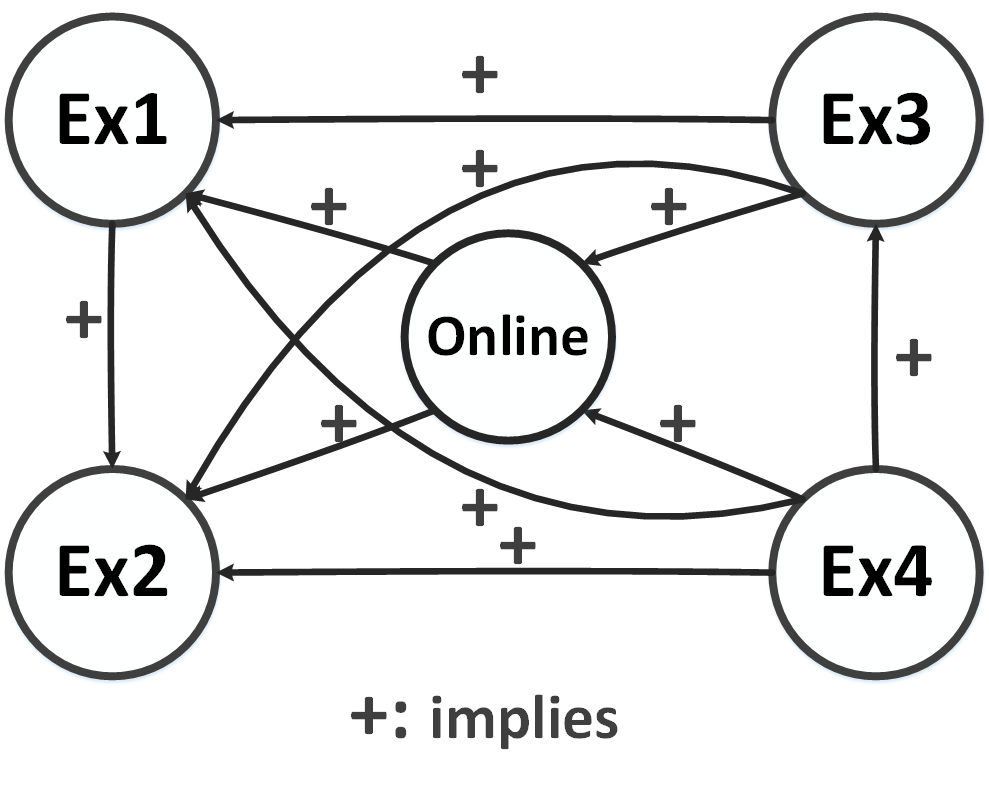
\includegraphics[scale=0.28]{figures/Fig8.png}}
	}}
      
      \caption{The implication relationships graph between existing observability 1, 2, 3, 4, and online observability where ``$\rightarrow$" means ``implies".}
      \label{fig:7}
   \end{figure}

From the implication relationships between online observability and existing observability we know that the online observability can help us solve some problem which can not be solved by existing observability. 
 \begin{itemize}
 \item Firstly, if the \BCNs\ are online observable but not satisfy the existing third and fourth observability, then the online observability can help us determine their initial state. 
 \item Secondly, it takes least observation costs for us to determine the initial state of some systems described by \BCNs. There are some biological systems depicted by \BCNs, such as the immune systems which can be depicted as the \BCN\ T-cell receptor kinetics model \cite{Klamt2006A}. And there exist input-nodes and state-nodes in this model, for the purpose of obtain the initial state of this \BCN, we must select some state-nodes to be observed at first. If we use the online observability to determine the initial state of the \BCN\ T-cell receptor kinetics model, then we need less output-nodes and then least observation costs.
 \end{itemize}

What is more, with the online observability, we can make some optimizations in the process of determining the initial state. We will represent them in the {\em Section \ref{sec:app}}.
   
   
%When I learned the four existing kinds of observability of \BCNs, I found that if we want to determine the initial state of a \BCN\ by first kind of observability, we need to guess the initial state of the \BCN\ and then check it by its corresponding input sequence. If the initial state we guess is right then we can determine the initial state of this \BCN. But if what we guess is incorrect, we need to guess the initial state again and use its corresponding input sequence to determine the initial state of this \BCN. We repeat this process untll we determine the initial state of this \BCN. But if we can not repeat this process, we can not determine the initial state of the \BCN\ too. Then I turned my gaze to the third observability, this kind of observability makes we can determine the initial state without presupposing the initial state. But I thought if we can determine the possible states set of the \BCN\ by observing the output at first, why do not we find corresponding input sequences for these possible states sets when we determine the initial state of \BCN? Compared with the existing third observability this method needs weaker preconditions of \BCNs\ for us to determine their initial state. Then I talked about this thinkness with my teacher, and we expand it into the original idea of the online observability of \BCNs. 
%==============================================================================================================